\documentclass[12pt,a4paper]{article}
%\usepackage[utf8]{inputenc}
%\usepackage[russian]{babel}
\usepackage{amsmath}
\usepackage{amsfonts}
\usepackage[pdftex]{graphics}
\DeclareGraphicsRule{*}{mps}{*}{}

\newcommand{\vc}{\overrightarrow}

\author{Portnov Ilya V.}
\title{Blending Bezier curve with continuous curvature}

\begin{document}
\maketitle

\section{Problem Statement}

Let's consider two curves:
$$
\varphi = \varphi(t),\quad t\in[0;1]
$$
and
$$
\psi = \psi(t),\quad t\in[0;1]
$$
in 3D space. We want to derive such a curve
$$
\gamma = \gamma(t), \quad t\in[0;1]
$$
that it has G2-continuous joints with the end of first curve ($\varphi$) and with the beginning of the second curve ($\psi$); more precisely, we want the curve $\gamma$ to have the following proerties:
\begin{enumerate}
  \item The end of $\varphi$ coincides with the beginning of $\gamma$, i.e.,
    \begin{equation}\label{C0}
    \gamma(0) = \varphi(1)
    \end{equation}
  \item Tangent vector of $\varphi$ at it's end is equal to tangent vector of $\gamma$ at it's beginning, i.e.,
    \begin{equation}\label{C1}
    \gamma'(0) = \varphi'(1)
    \end{equation}
  \item Normal vector of $\varphi$ at it's end is pointing in the same direction as the normal vector of $\gamma$ at it's beginning. I.e.,
    \begin{equation}\label{normal}
    \mathbf{n}(\gamma)(0) \parallel \mathbf{n}(\varphi)(1)
    \end{equation}
    (we use $\mathbf{n}(\gamma)$ to denote the normal vector of the curve).
  \item $\gamma$ curve has the same curvature at it's beginning, as $\varphi$ has at it's end, i.e.,
    \begin{equation}\label{curvature}
    \kappa(\gamma)(0) = \kappa(\varphi)(1)
    \end{equation}
    (we use $\kappa(\gamma)$ to denote the curvature of the curve).
  \item The same goes for joining of $\gamma$ with $\psi$.
\end{enumerate}

Obviously, there are a lot of curves that satisfy these conditions. But in addition, we want our curve $\gamma$ to be a Bezier curve. We will show that to satisfy these conditions, it is enough to use Bezier curve of 5th degree (with 6 control points). We will search our curve in the following form:
\begin{equation}\label{bezier}
\gamma(t) = A_1(1-t)^5 + 5B_1(1-t)^4t + 10C_1(1-t)^3t^2 + 10C_2(1-t)^2t^3 + 5B_2(1-t)t^4 + A_2t^5
\end{equation}
Here $A_1$, $A_2$, $B_1$, $B_2$, $C_1$ and $C_2$ are control points of our Bezier curve. They are to be found.

\section{A note on problem statement}
One may note, that it is always possible to replace our equations \eqref{normal} and \eqref{curvature} with
\begin{equation}\label{C2}
\gamma''(0) = \varphi''(1)
\end{equation}
(this is what called C2 continuity).
Then from equations \eqref{C0}, \eqref{C1} and \eqref{C2} it would be quite simple to derive equations for our control points. However, the equation \eqref{C2} is more strong than \eqref{normal} and \eqref{curvature}, as we will see in details later. If we experiment a bit with C2 continuity, we will see, that geometrically makes our blending curve follow the "inertia" of $\varphi$ and $\psi$ very strongly, and thus, the blending curve with C2 continuity can be bent too much in order to look "naturally". Figure \ref{fig:C2} illustrates what we mean.

\section{Determining first two pairs of control points}

First, from \eqref{C0} and \eqref{bezier} we can obviously state that
$$
A_1 = \varphi(1),\quad A_2 = \psi(0)
$$
To simplify the notation, we will just note that $\gamma(0)$, $\gamma(1)$, $\gamma'(0)$ and $\gamma'(1)$ are known to us, and later we will use these notations instead of $\varphi$ and $\psi$. For example, the previous equation we may write as:
\begin{equation}
A_1 = \gamma(0), \quad A_2 = \gamma(1)
\end{equation}

Now, if we write down the formula for the first derivative of our Bezier curve at $t = 0$, it will be pretty simple:
\begin{equation}
\gamma'(0) = 5(B_1 - A_1)
\end{equation}
The formula for the first derivative at $t = 1$ will look similar:
\begin{equation}
\gamma'(1) = 5(A_2 - B_2)
\end{equation}
So, now we know two more control points:
\begin{equation}
B_1 = A_1 + \frac{1}{5}\gamma'(0) \quad B_2 = A_2 - \frac{1}{5}\gamma'(1)
\end{equation}

\section{Determining $C_1$ and $C_2$}

We have used two more or less trivial of our equations and found four control points. Now we have to use equations \eqref{normal} and \eqref{curvature} to find $C_1$ and $C_2$. We will concentrate on finding $C_1$, as formulas for $C_2$ can be obviously found from symmetry. To simplify notation, we will omit the lower indexes, and write $A$, $B$ and $C$ for $A_1$, $B_1$ and $C_1$. We will write indexes only when it is necessary to avoid confusion.

Let's start with writing down formulas for curvature and normal:

\begin{equation}\label{curvature:def}
\kappa = \frac{|\gamma' \times \gamma''|}{|\gamma'|^3}
\end{equation}

\begin{equation}\label{normal:def}
\mathbf{n} = (\gamma' \times \gamma'') \times \gamma'
\end{equation}

(we use $\times$ for vector cross product). Let's also write down the formula for the second derivative of our curve at $t = 0$:
\begin{equation}\label{secondderivative}
\gamma''(0) = 20(A - 2B + C)
\end{equation}

We see that both equations for $\kappa$ and $\mathbf{n}$ contain $\gamma'\times\gamma''$. Let's calculate this product at $t=0$:
\begin{multline*}
\gamma'(0)\times\gamma''(0) = 5(B-A) \times 20 (A - 2B + C) = \\
= 100 (B\times A - 2B\times B + B\times C - A\times A + 2 A\times B - A\times C) = \\
= 100 (B\times A + B\times C + 2A\times B - A\times C) = \\
= 100 (A\times B + B\times C - A\times C)
\end{multline*}

Now we are going to simplify things even further. We know that Bezier curves have the property of translational invariance; i.e., if we move all control points by some vector, we will have the same curve, just moved by the same vector. So, let's substract the vector $A$ from all our control points (we will just have to remember to add it back in the end). We thus will replace $A$ with $0$, $B$ with $\vc{AB}$, and $C$ with $\vc{AC}$. This way we will have a simple formula:
\begin{equation}
\gamma'(0)\times\gamma''(0) = 100(\vc{AB}\times\vc{AC})
\end{equation}
Now, if we remember the definition of vector cross product in 3D space, we can rewrite \eqref{curvature:def} as
$$
100|\vc{AB}||\vc{AC}|\sin\angle CAB = \kappa(\gamma)(0)|\gamma'(0)|^3
$$
or, if we remember that $|\vc{AB}| = |\gamma'(0)|/5$,
\begin{equation}\label{star2}
  |\vc{AC}|\sin\angle CAB = \frac{1}{20}\kappa(\gamma)(0)|\gamma'(0)|^2
\end{equation}
Here we know everything on the right side, and we do not know $|\vc{AC}|$ and $\angle CAB$ on the left side.
This equation has interesting geometric meaning: it means that $C$ lies on some line $l$, which is parallel to $(AB)$, and distance between $l$ and $(AB)$ is $d = \frac{1}{20}\kappa(\gamma)(0)|\gamma'(0)|^2$ (this should be clear from fig.\ref{fig:points}).

\begin{figure}[h]
  \caption{Relations between control points $A$, $B$ and $C$}
  \label{fig:points}
  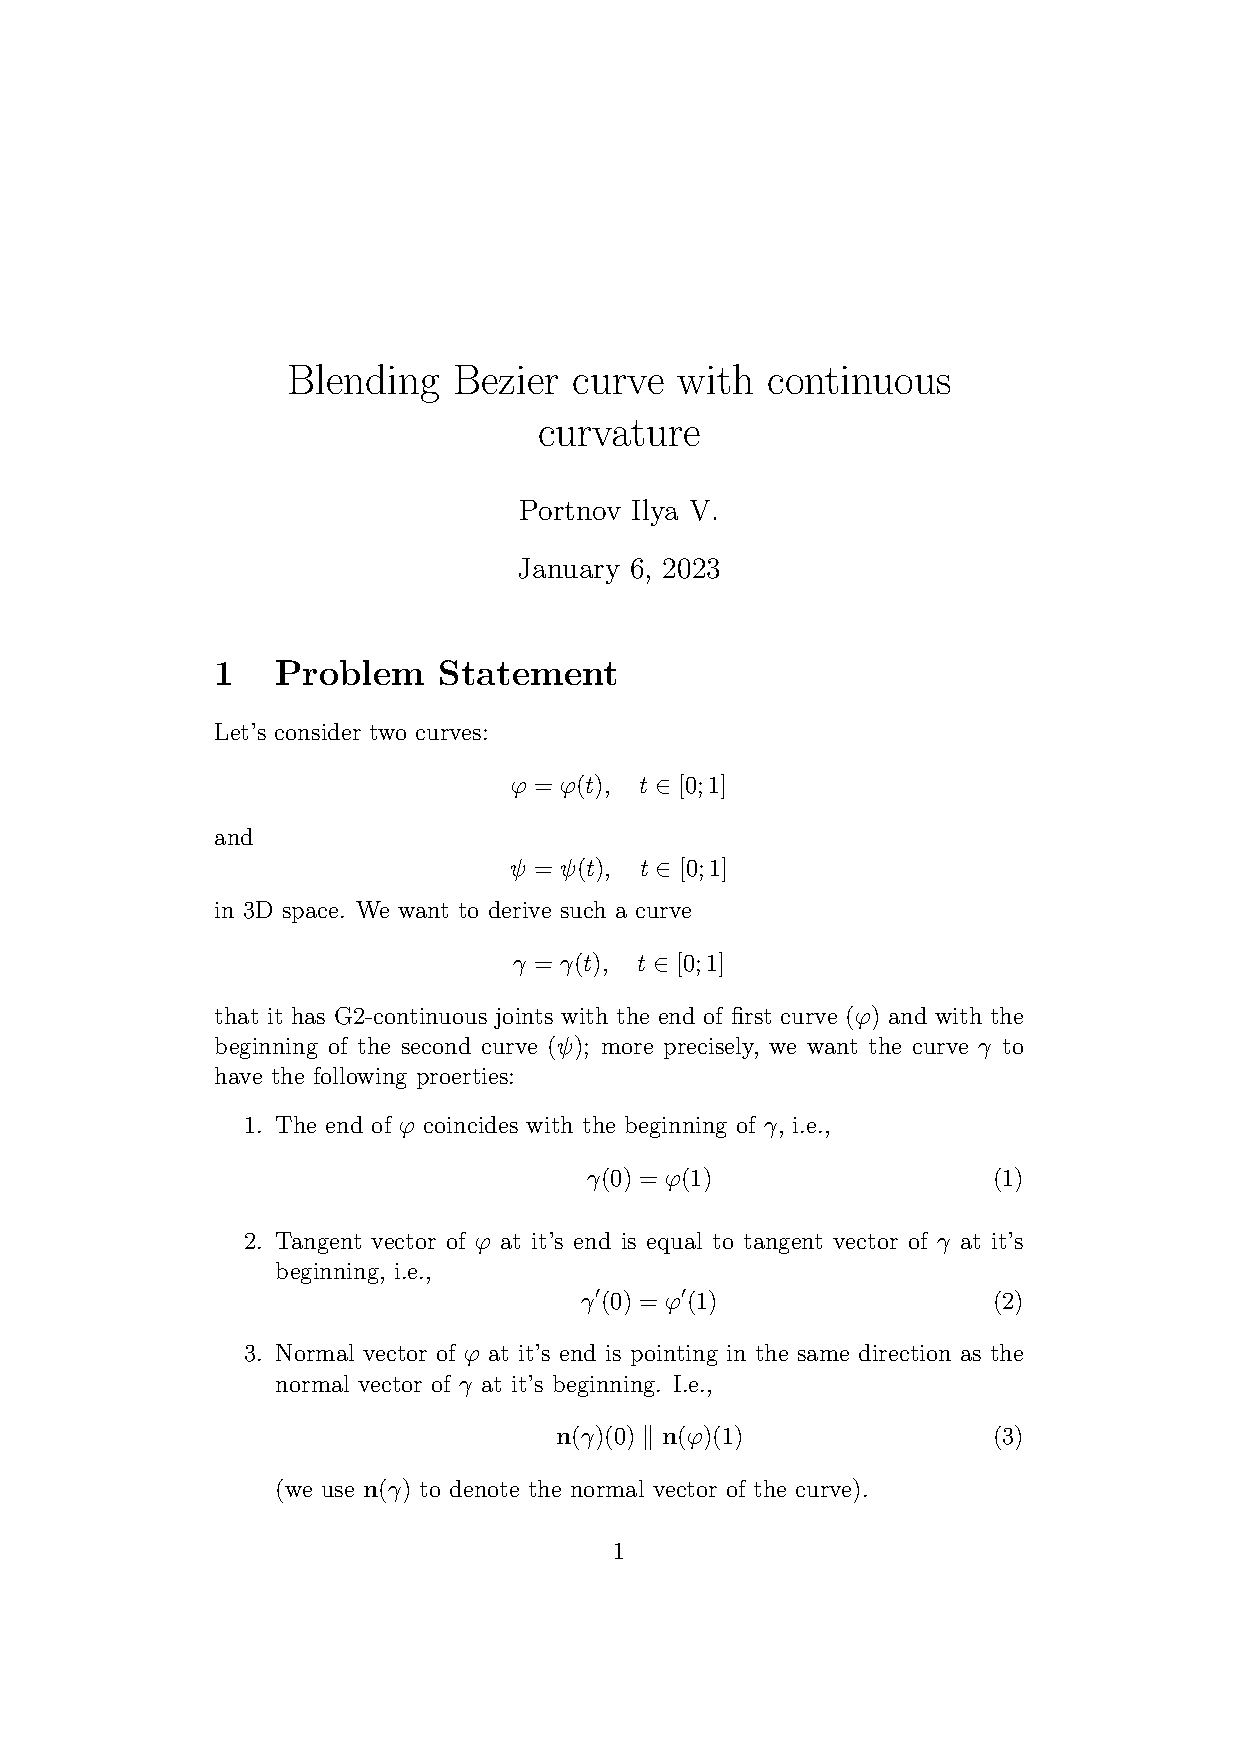
\includegraphics{bezier5.2}
  \centering
\end{figure}

Also we know that $C$ lies in the plane, which goes through point $A$ and $B$, and contains the $\mathbf{n}(\gamma)(0)$ vector (this is clear from \eqref{secondderivative}). So we already know how to draw the line $l$: we should draw a line which is parallel to $(AB)$, lies in the plane $(A, B, A + \mathbf{n}(\gamma)(0))$, and has distance from $(AB)$ equal to $d$. Now the remaining question is where exactly on that line should we place our point $C$. Any point on line $l$ will satisfy conditions \eqref{C0} -- \eqref{curvature}. To select a specific point, we should add some additional condition.

Obviously we can invent different conditions for location of $C$. For example,
\begin{enumerate}
  \item we can simply let $\vc{BC}$ be parallel to $\mathbf{n}(\gamma)(0)$, i.e. let $C = B + d\mathbf{n}(\gamma)(0)$. There is no clear geometrical reason for this, but this is computationally the simplest idea.
  \item Or we can say that we want to minimize $|\gamma''(0)|$.
  \item Or we may want $C$ to lie somewhere near the line $(B_1B_2)$ -- as near as possible. Some experiments show that this tends to give nice enough curves.
\end{enumerate}

\section{Minimizing $|\gamma''(0)|$}

Let's consider the second condition. From \eqref{secondderivative}, we can write the second derivative of $\gamma$ at $t=0$ as
$$
\gamma''(0) = 20(\vc{AC} - 2\vc{AB}).
$$
From this equation it is clear that if we want to minimize $|\gamma''(0)|$, we need to make $C$ as close to $A + 2\vc{AB}$ as possible, while remaining on the line $l$. This is achieved when $A + 2\vc{AB}$ is the projection of $C$ to $(AB)$ line (refer to fig. \ref{fig:minimize}).

\begin{figure}[h]
  \caption{Minimizing the second derivative}
  \label{fig:minimize}
  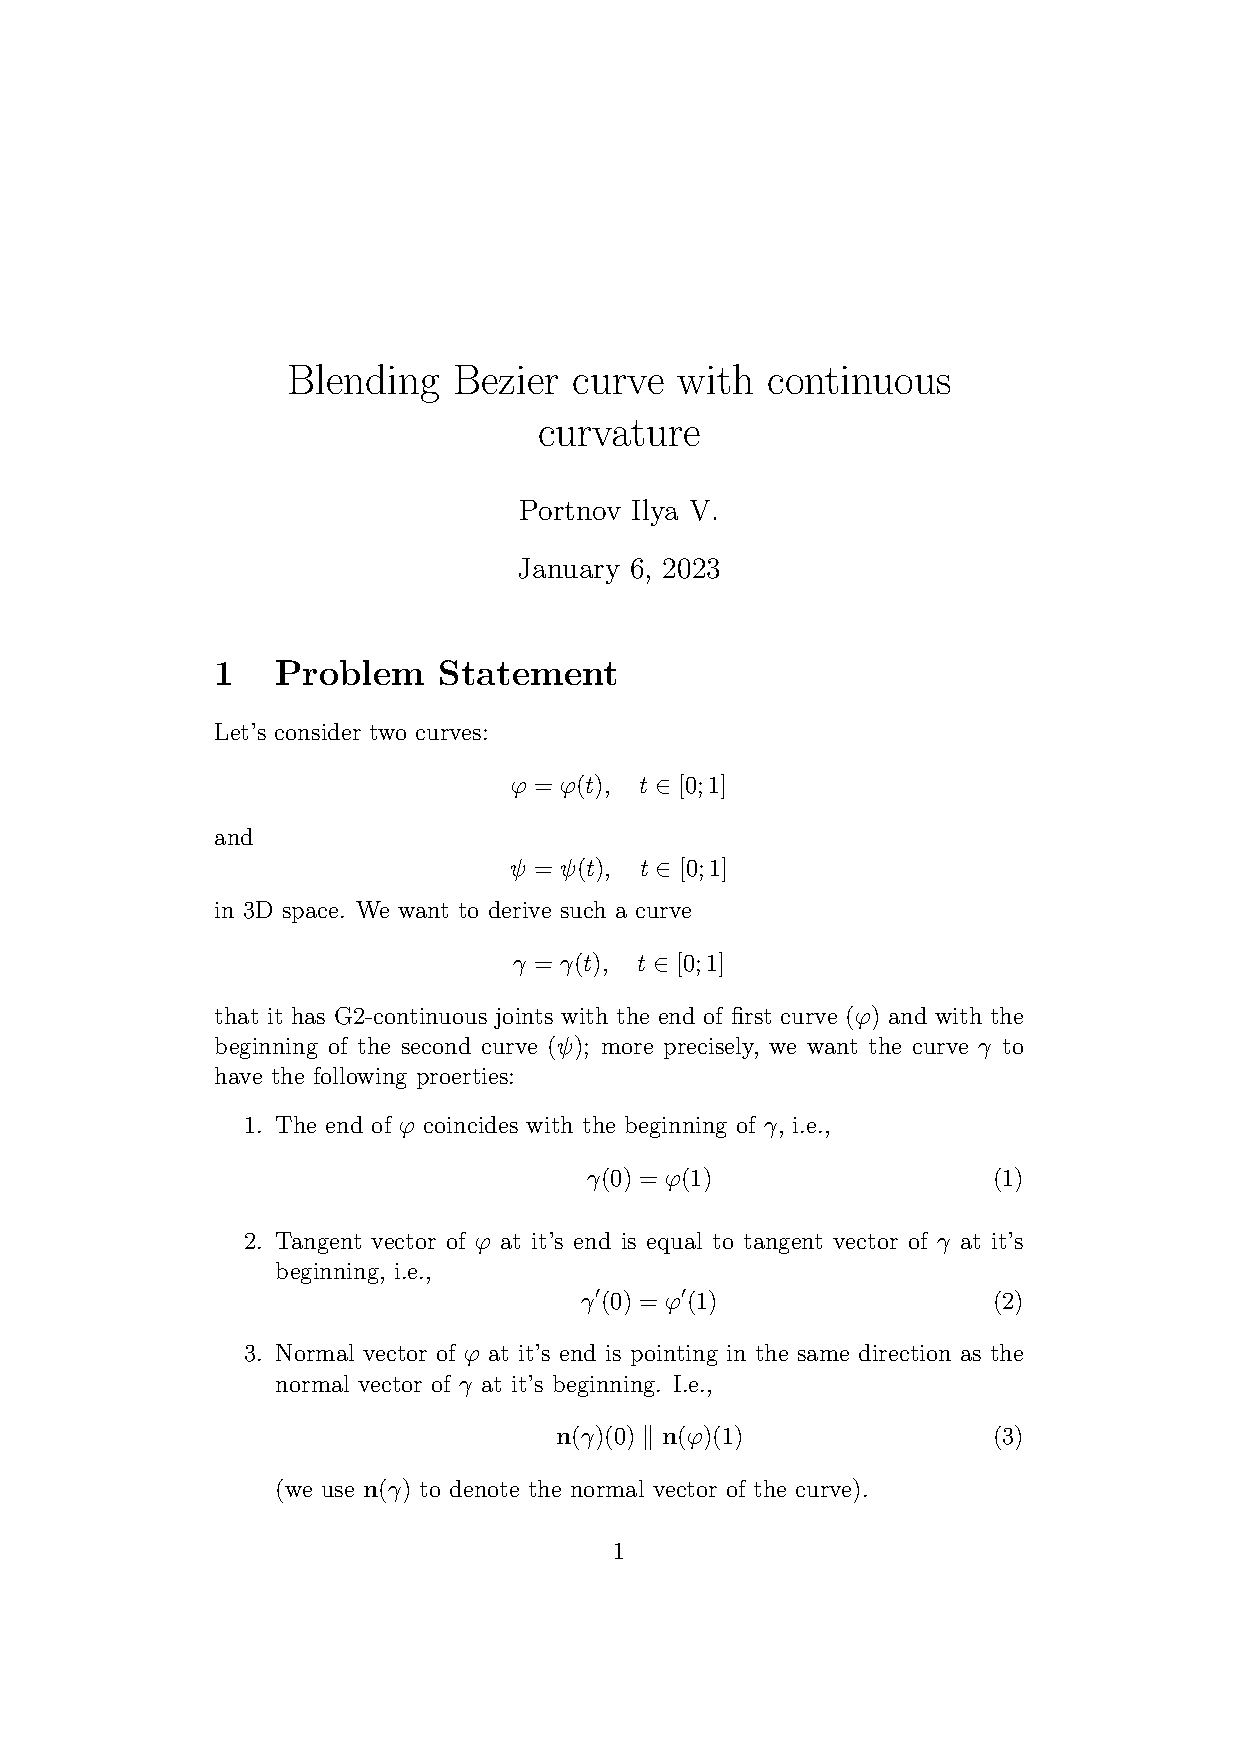
\includegraphics{bezier5.3}
  \centering
\end{figure}

From the same picture it is now clear that in such a case we can write $C$ as
\begin{equation}\label{Cbyminimize}
  C = B + \vc{AB} + d\mathbf{n}(\gamma)(0)
\end{equation}

Figure \ref{fig:minimizedCurve} is the example of what these formulas give for the same initial curves that were used for fig.\ref{fig:C2}.

\section{Putting $C$ near $(B_1B_2)$ line}

We will now concentrate on the latest condition.

\begin{figure}[h]
  \caption{Location of point $C$ near $(B_1B_2)$ line}
  \label{fig:nearest}
  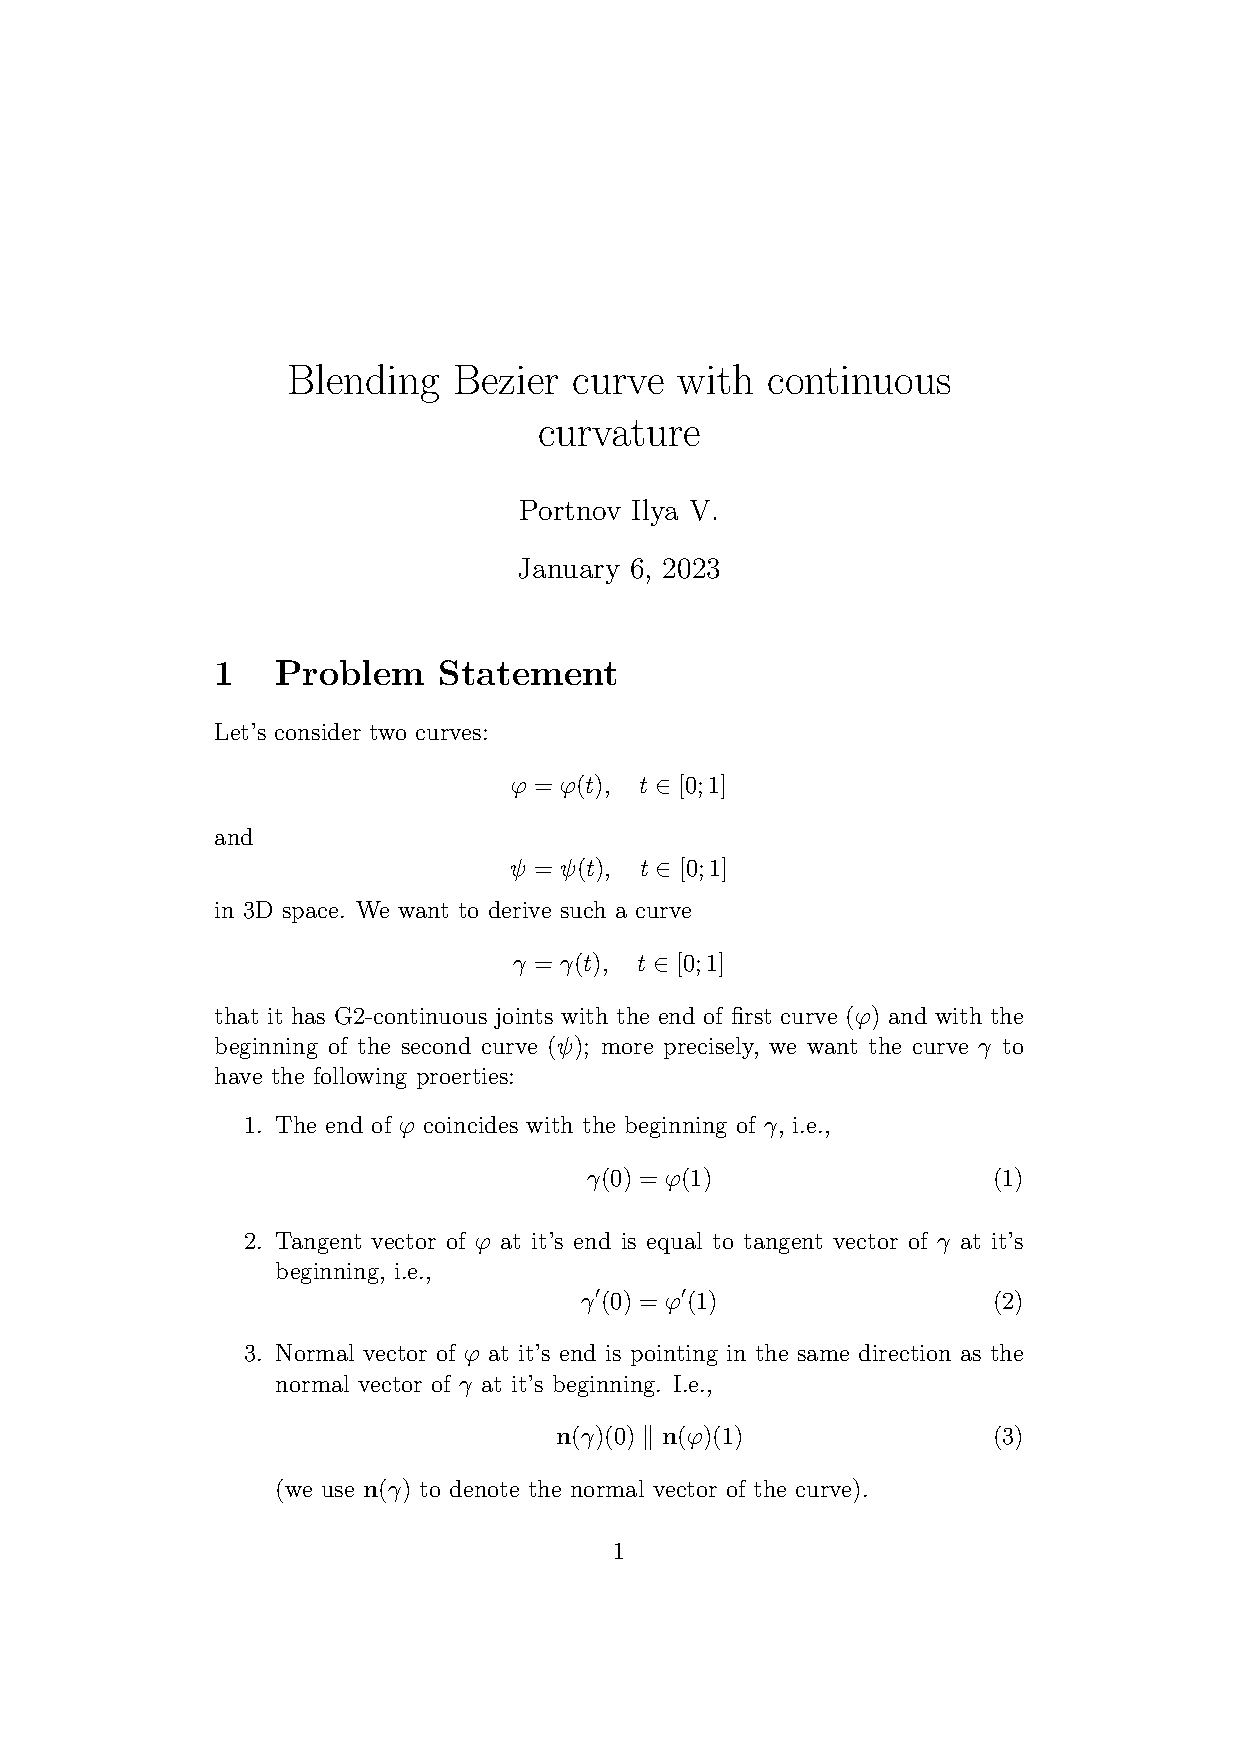
\includegraphics{bezier5.4}
  \centering
\end{figure}

In fact, what we want is $C$ to be the nearest point on line $l$ to the line $(B_1B_2)$. For this to take place, there should be the following conditions met:
\begin{enumerate}
  \item $\angle B_1C_0C$, where $C_0$ is defined as the nearest point on $l$ to $(AB)$, should be a right angle;
  \item $\angle B_1HC$, where $H$ is defined as the nearest point on $(B_1B_2)$ to $l$, should be a right angle.
\end{enumerate}
We can rewrite these conditions in terms of vector scalar products:
\begin{equation}\label{scalarC}
(C_0C, HC) = 0
\end{equation}
and
\begin{equation}\label{scalarH}
(HC, B_1H) = 0
\end{equation}
These equations can be solved algebraically. Let's define vector $\vec a$ as a unit vector in the same direction as $\vc{AB}$, and vector $\vec b$ as a unit vector in the same direction as $\vc{B_1B_2}$. Then we can state that there exist such numbers $t_1$ and $t_2$, that
\begin{equation}\label{Cfromt1}
C = C_0 + t_1\vec{a}
\end{equation}
and
$$
H = B_1 + t_2\vec{b}
$$
Also we should remember that
$$
C_0 = B_1 + d\mathbf{n}(\gamma)(0)
$$
Now we can rewrite \eqref{scalarC} as
$$
(t_1\vec{a}, d\mathbf{n} + t_1\vec{a} - t_2\vec{b}) = 0
$$
Expanding the parentheses in the left-hand side, we will have
$$
  (t_1\vec{a}, d\mathbf{n}) + (t_1\vec{a}, t_1\vec{a}) - (t_1\vec{a}, t_2\vec{b}) = 0
$$
or, remembering that $\vec{a}$ is orthogonal to $\mathbf{n}$,
$$
(t_1\vec{a}, t_1\vec{a}) = (t_1\vec{a}, t_2\vec{b}).
$$
Now if we expand the definition of scalar product and remember that $\vec{a}$ and $\vec{b}$ are unit vectors, we will have
$$
t_1^2 = t_1t_2\cos(\widehat{\vec{a}, \vec{b}}) = t_1t_2(\vec{a}, \vec{b})
$$
or, dividing by $t_1$, simply
\begin{equation}\label{t1}
t_1 = t_2(\vec{a}, \vec{b}).
\end{equation}
Now let's return to equation \eqref{scalarH}. Similarly, we will have
$$
(d\mathbf{n} + t_1\vec{a} - t_2\vec{b}, t_2\vec{b}) = 0,
$$
or
$$
(d\mathbf{n}, t_2\vec{b}) + (t_1\vec{a}, t_2\vec{b}) - (t_2\vec{b}, t_2\vec{b}) = 0,
$$
or (remembering that $\vec{b}$ is a unit vector)
$$
dt_2(\mathbf{n},\vec{b}) + t_1t_2(\vec{a}, \vec{b}) = t_2^2,
$$
or (dividing by $t_2$)
\begin{equation}\label{t2viaH}
d(\mathbf{n}, \vec{b}) + t_1(\vec{a}, \vec{b}) = t_2.
\end{equation}
Subsitituting $t_1$ from \eqref{t1} into \eqref{t2viaH}, we will have
$$
d(\mathbf{n}, \vec{b}) + t_2(\vec{a}, \vec{b})^2 = t_2.
$$
Now we can express $t_2$ as
\begin{equation}\label{t2}
  t_2 = \frac{d(\mathbf{n}, \vec{b})}{1 - (\vec{a}, \vec{b})^2}.
\end{equation}
(Side note: the denominator in the last equation is exactly $\sin^2(\widehat{\vec{a}, \vec{b}})$).

So, finally, subsituting \eqref{t2} and \eqref{t1} into \eqref{Cfromt1}, we have
\begin{equation}
  C = B_1 + d\mathbf{n} + d\frac{(\vec{a}, \vec{b})(\mathbf{n}, \vec{b})}{1 - (\vec{a}, \vec{b})^2}\vec{a}
\end{equation}

Figure \ref{fig:b1b2} is the example of what these formulas give for the same initial curves that were used for fig.\ref{fig:C2}.

\section{Resulting blending curves}

The following figures show what kind of curves are received by using different approaches we discussed above.

\begin{figure}[h]
  \caption{C2-continuous blending of two curves}
  \label{fig:C2}
  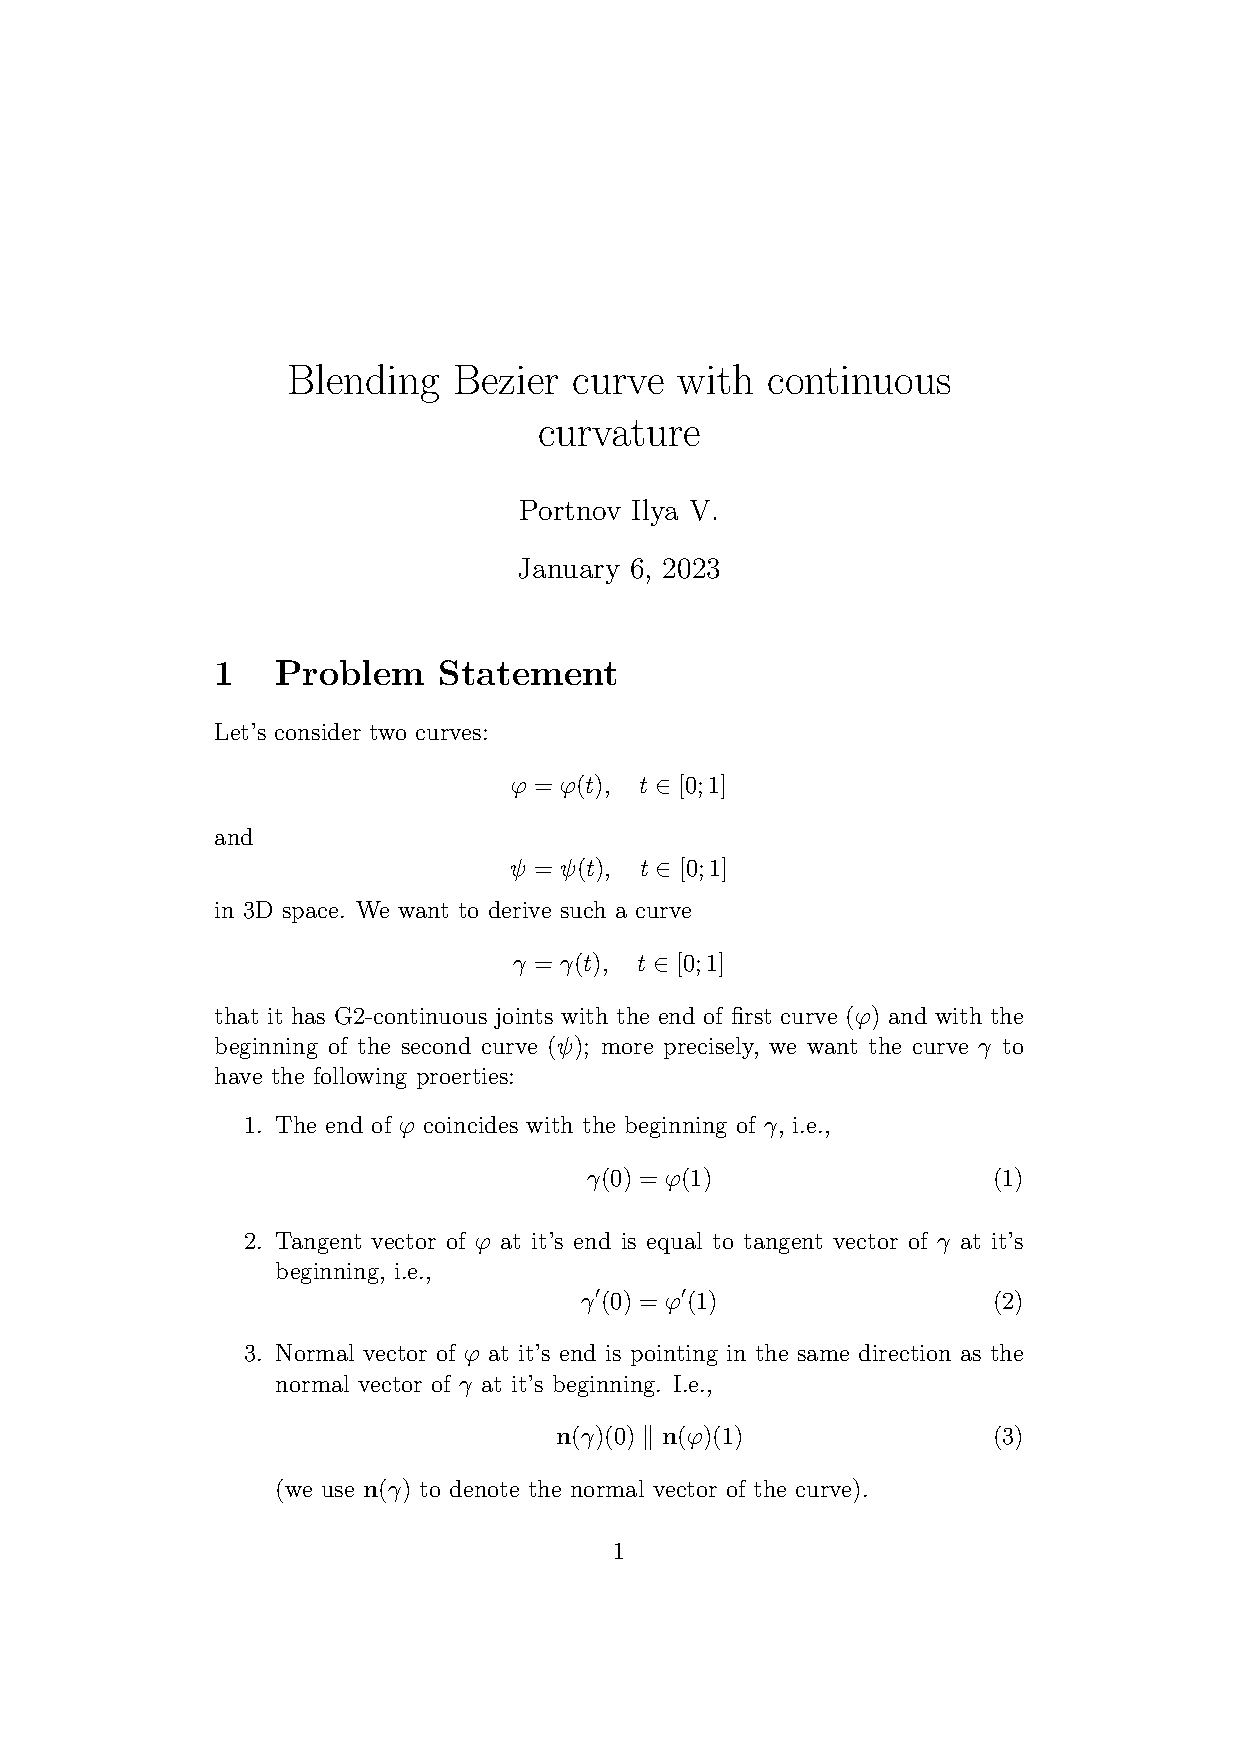
\includegraphics{bezier5.1}
  \centering
\end{figure}

\begin{figure}[ht]
  \caption{G2-continous blending of two curves, second derivative minimized}
  \label{fig:minimizedCurve}
  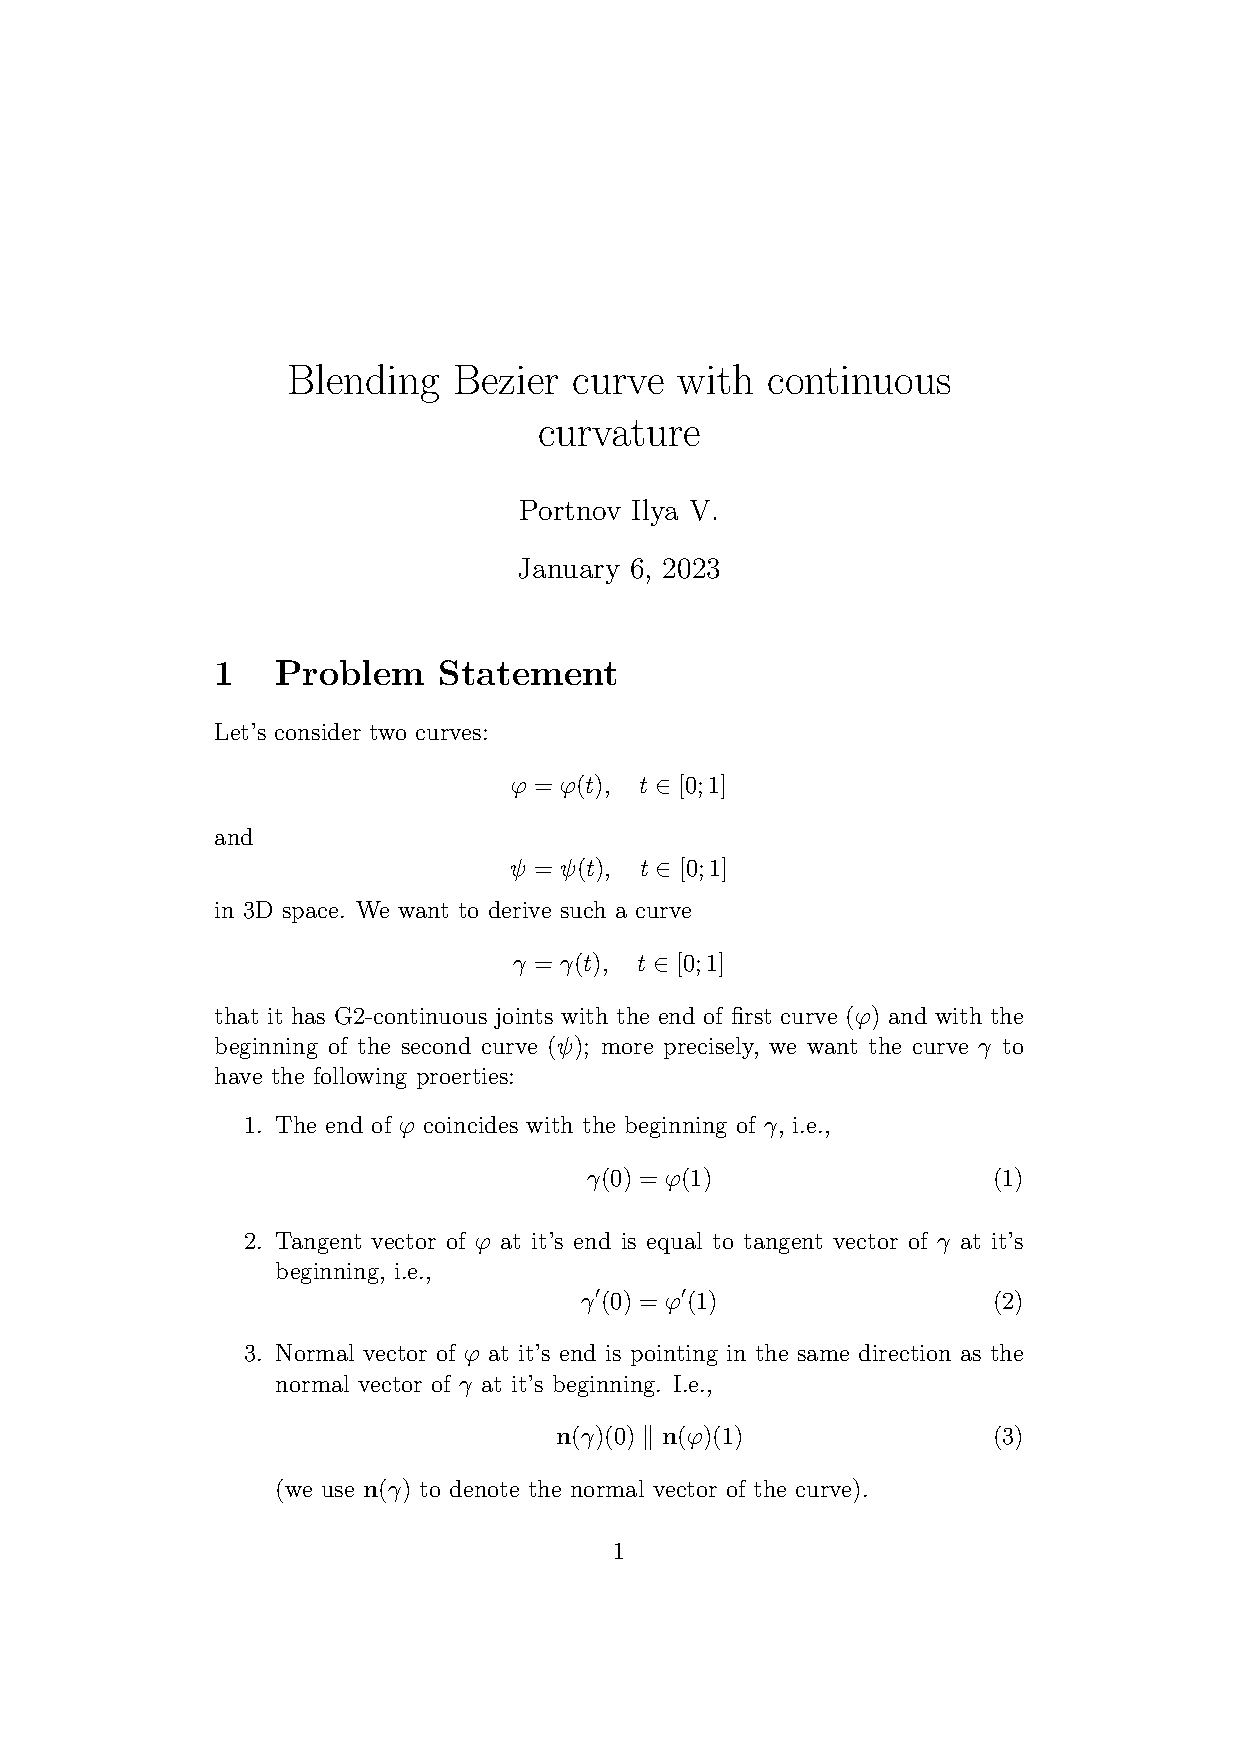
\includegraphics{bezier5.5}
  \centering
\end{figure}

\begin{figure}[ht]
  \caption{G2-continous blending of two curves, $C$ points aligned by $(B_1B_2)$}
  \label{fig:b1b2}
  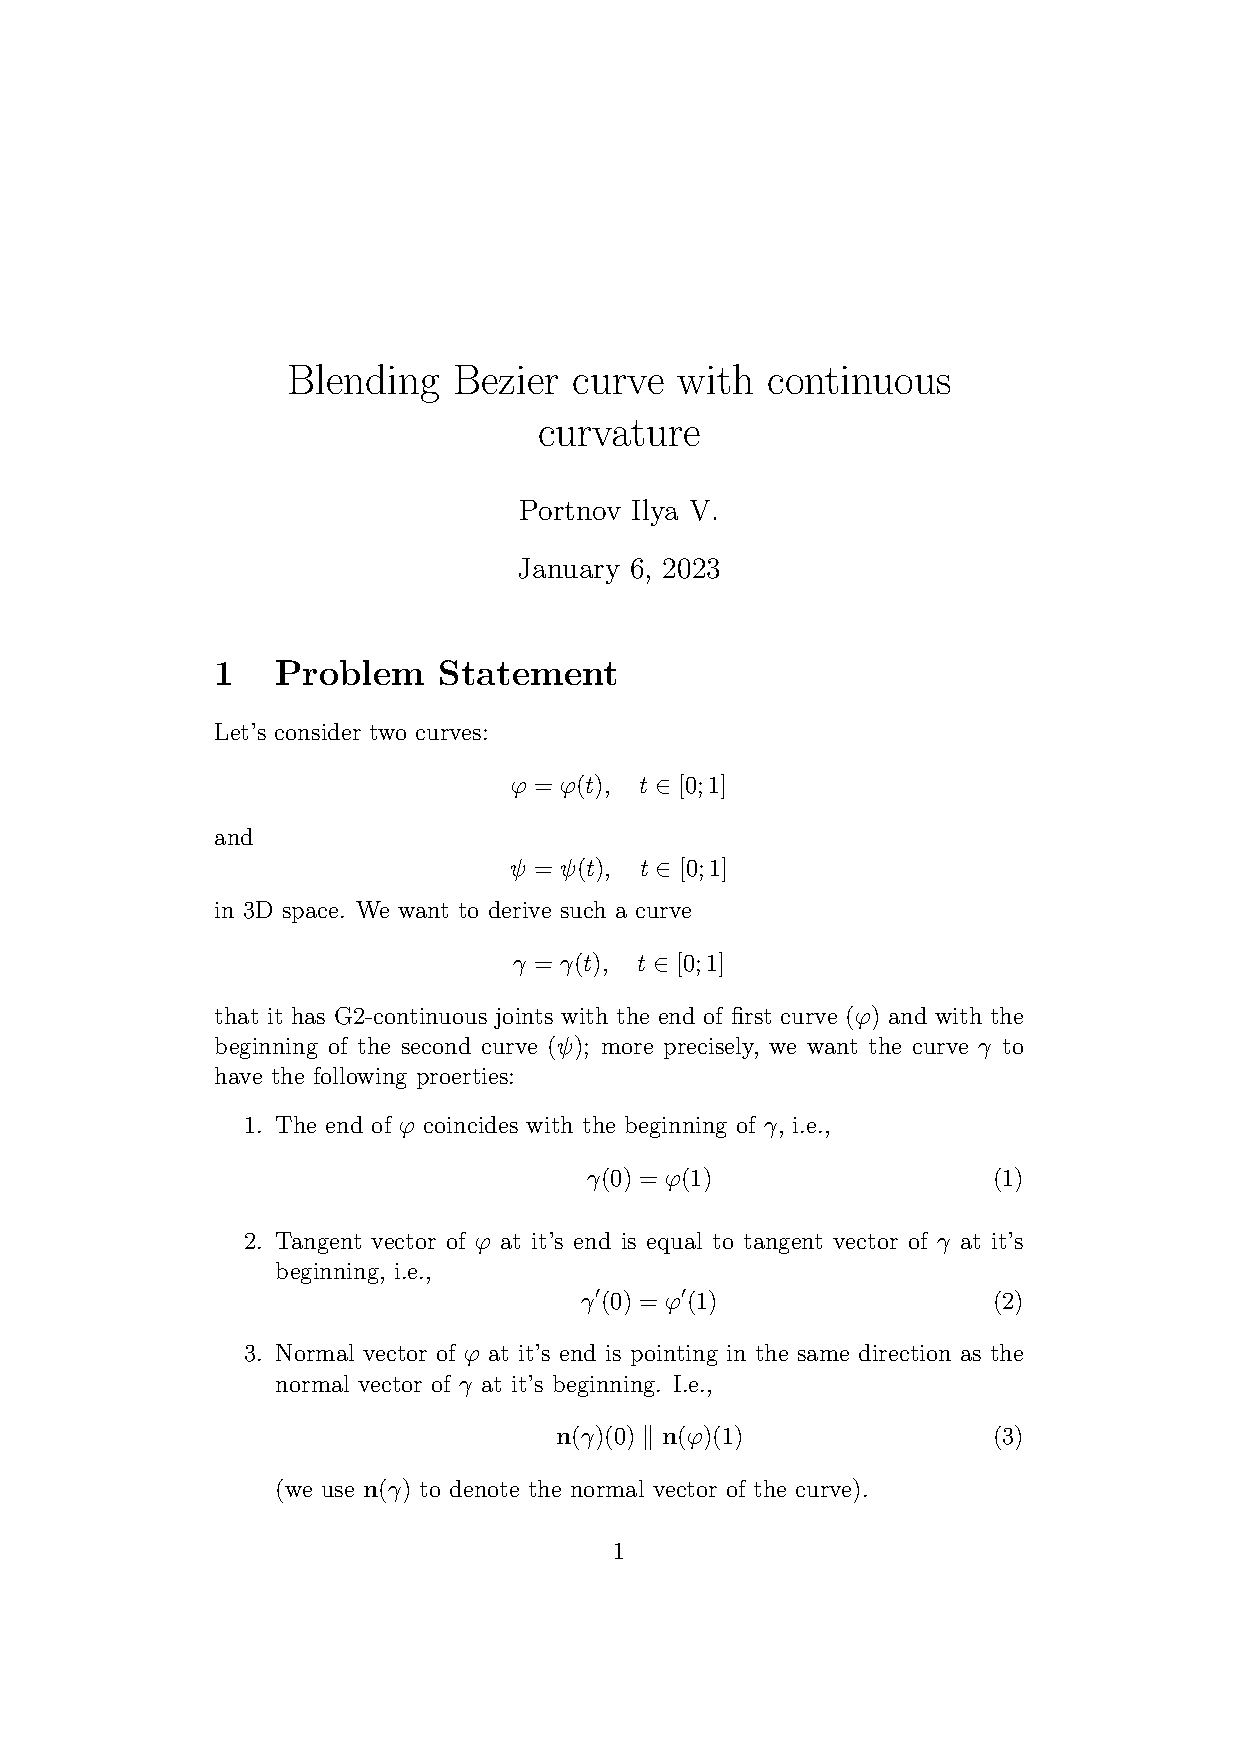
\includegraphics{bezier5.6}
  \centering
\end{figure}

\end{document}
